\scanpage{64}
% archive foliation: 63
\unsure{soient|sont} des isomorphismes, avec le complément que $\uline{H^{\unsure{0|i}}(X,M)\text{ est un}}$ $\mathbf{Q}$-\uline{module de type fini}.
\figure{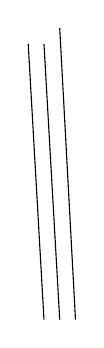
\begin{tikzpicture}[x=1mm,y=1mm]\draw (0,0)--(-2,35);\draw (2,0)--(0,35);\draw (4,0)--(2,37);\end{tikzpicture}}

\deleted{Ceci doit être valable en particulier dans les deux cas \unsure{typiques} suivants
\[
\begin{array}{ll}
\text{a)}&X\text{ de type fini sur }\mathbf{Z}\\
\text{b)}&X\text{ de type fini sur un corps alg. clos.}
\end{array}
\]}

En particulier, pour un corps alg. clos $k$, on aura
\[
H^i(k,M)=0\quad\text{pour }i>0,\qquad \forall\text{ motif }M.
\]

\uline{NB} Si $X$ est de type fini ($=$ projectif lisse) sur un corps alg. clos $K$, \unsure{on n'a plus de} telles relations précises, comme on voit par calcul explicite (utilisant les conjectures de Tate) pour $K$ clôture algébrique d'un corps fini ----

Le th de Tate peut se reformuler et se préciser en énonçant :
\[
A^i(X)\otimes_{\mathbf{Z}}\mathbf{Q}\inserted{\nearrow\ \unsure{\text{pas}|\text{pr}}\ \mathbf{Q}_\ell}\simeq \Gamma_k(R^i f_*(\mathbf{Q}_X(\unsure{i|0})))
\]
